\chapter{Proof-of-Concept}%
\label{ch:poc}
Voor het eerste praktische deel van deze bachelorproef werden er drie virtuele machines opgezet binnen VirtualBox met behulp van Vagrant om een gecontroleerde testomgeving te creëren. Deze virtuele machines (VM’s) simuleren een scenario waarin een ransomware-aanval gericht wordt op databases die door het bedrijf worden beheerd. Het primaire doel van deze simulatie is aan te tonen dat het gebruik van immutable storage een effectieve maatregel kan zijn om belangrijke data te beschermen tegen ransomware-aanvallen.
\subsection{Relevantie van de PoC voor de Azure-omgeving van Forvis Mazars}
De Proof-of-Concept (PoC) in VirtualBox simuleert een ransomware-aanval in een lokale omgeving, gericht op het evalueren van beveiligingsmaatregelen zoals immutable storage. Deze aanpak sluit nauw aan bij de Azure-omgeving van Forvis Mazars, waar databases en back-ups worden beheerd.

De technieken uit de PoC, zoals immutable storage, kunnen direct worden toegepast in Azure via functies zoals immutable blobs in Azure Storage. Dit maakt het mogelijk om gegevens beter te beschermen tegen wijzigingen of verwijdering. Daarnaast biedt de PoC een veilig platform om de impact van een ransomware-aanval te begrijpen en te testen hoe snel en effectief back-ups kunnen worden hersteld, wat een cruciaal aspect is voor de bedrijfscontinuïteit.

Forvis Mazars kan de PoC gebruiken om risico’s te analyseren en beveiligingsoplossingen eerst kleinschalig te testen, alvorens deze op grotere schaal binnen hun cloudinfrastructuur toe te passen. Hiermee helpt de PoC bij het verfijnen en optimaliseren van hun bestaande Azure-back-upstrategie.
\subsection{Technische uitwerking}
Voor het opzetten van de virtuele machines in de Proof-of-Concept (PoC) werd gebruik gemaakt van een Vagrantfile, zie bijlage \ref{sec:vagrant}, die de specificaties en configuraties van de VM’s bepaalt.

In de onderstaande tabel worden de specificaties van de drie virtuele machines weergegeven die in de Proof-of-Concept zijn gebruikt. Elke VM heeft een specifieke functie binnen het netwerk. De tabel bevat details over de hoeveelheid toegewezen RAM, het aantal CPU-cores, het gebruikte besturingssysteem, de toegewezen IP-adressen en de configuratie van de netwerkadapter. Deze configuratie zorgt ervoor dat de VM's binnen hetzelfde interne netwerk met elkaar kunnen communiceren, wat essentieel is voor het testen van de ransomware-aanval en de back-upstrategieën.
\begin{longtable}{|l|c|c|c|l|l|}
    \hline
    \textbf{Functie} & \textbf{RAM} & \textbf{CPU Cores} & \textbf{IP} & \textbf{Besturingssysteem} & \textbf{Netwerkadapter} \\ \hline
    Primary server    & 2 GB         & 1                  & 192.168.0.10 & Ubuntu 22.04.5 LTS & NAT + Internal \\ \hline
    Back-up server           & 1 GB         & 1                  & 192.168.0.20 & Ubuntu 22.04.5 LTS & NAT + Internal \\ \hline
    Attacker VM         & 2 GB         & 1                  & 192.168.0.30 & Ubuntu 22.04.5 LTS     & NAT + Internal \\ \hline
    
\caption{Beschrijving van de virtuele machines in de Proof of Concept}
\end{longtable}

De Primary VM stelt een actieve databankserver voor binnen een bedrijfsomgeving. Deze server bevat de operationele data en vertegenwoordigt de belangrijkste bron die beschermd moet worden tegen dataverlies of aanvallen. 

De Back-up VM fungeert als een back-upserver waarop regelmatig de back-ups worden opgeslagen. Deze back-upserver is cruciaal voor bedrijfscontinuïteit en disaster recovery, omdat ze in geval van een aanval of fout de herstelmogelijkheden biedt. 

De Attacker VM vertegenwoordigt een hacker met slechte intenties binnen de testomgeving. Deze machine wordt gebruikt om een ransomware-aanval te simuleren, waarbij de functionaliteit van zowel de Primary VM als de Back-up VM wordt bedreigd. 

Het doel van deze opstelling is om te demonstreren hoe immutable storage een bedrijf kan beschermen tegen de gevolgen van een ransomware-aanval.
\subsubsection{Aanmaken van de database}
Op de primary VM werd een eenvoudige SQL-database geïnstalleerd en de volgende tabel aangemaakt om als testdata te dienen:
\begin{lstlisting}[language=SQL, caption={MySQL-code voor het aanmaken van de testdatabank.}]
CREATE TABLE employees (
    id INT AUTO_INCREMENT PRIMARY KEY,
    name VARCHAR(50),
    role VARCHAR(50)
);
INSERT INTO employees (name, role) VALUES 
    ('Alice', 'Engineer'), 
    ('Bob', 'Manager'), 
    ('Charlie', 'Analyst');
\end{lstlisting}



\subsubsection{Back-up van de database}
Nadien werd de database geëxporteerd naar een \texttt{.sql}-bestand met het volgende \texttt{mysqldump}-commando:
\begin{lstlisting}[language=script, caption={Mysqldump commando om een databank te exporteren.}]
mysqldump -u testuser -p testdb > /home/vagrant/backup.sql
\end{lstlisting}
Het resulterende bestand, \texttt{backup.sql}, werd vervolgens met BorgBackup opgeslagen in een back-uprepository op de back-up VM. De repository werd vooraf geïnitialiseerd met het volgende commando:
\begin{lstlisting}[language=script, caption={Borg commando om een map te initialiseren als Borg repository.}]
borg init --encryption=repokey /home/vagrant/backups
\end{lstlisting}
Vervolgens werd de back-up gemaakt:
\begin{lstlisting}[language=script, caption={Borg commando om een back-up te nemen.}]
borg create --progress 
ssh://vagrant@192.168.0.20/home/vagrant/backups::backup-$(date +%Y-%m-%d) 
/home/vagrant/backup.sql
\end{lstlisting}

\subsubsection{Beveiliging van de back-up directory}
Om de back-up directory ransomware-resistent te maken, werd het Linux-commando \texttt{chattr} gebruikt om het \textit{immutable}-attribuut toe te passen op de back-up directory. Dit attribuut zorgt ervoor dat er geen wijzigingen aan de bestanden in de directory kunnen gebeuren, zelfs door gebruikers met \texttt{root}-rechten. Het commando:
\begin{lstlisting}[language=script, caption={Linux commando om de map immutable te maken.}]
sudo chattr +i /home/vagrant/backups/
\end{lstlisting}

\subsubsection{Simulatie van de ransomware-aanval}
Op de aanvaller-VM werd een script gebruikt om de ransomware-aanval te simuleren. Het script probeert alle bestanden in de back-up directory te versleutelen met behulp van een versleutelingstechniek (AES-256-CBC) door de inhoud van de bestanden te encrypteren en op te slaan met de extensie .enc. Na het encrypteren worden de oude bestanden verwijderd zodat deze niet meer bereikbaar zijn. Dit simuleert een ransomware-aanval waarbij de back-upbestanden worden versleuteld, waardoor ze niet meer bruikbaar zijn zonder het juiste decryptiesleutel. Zie bijlage \ref{sec:bash} voor de code van het script dat de aanval uitvoert.

Voor het gemak heeft de Attacker VM volledige controle gekregen over de back-up VM en de primary VM. Dit is gedaan omdat de scope van deze bachelorproef niet is om toegang te verkrijgen tot een server, maar eerder om een gecontroleerde omgeving te creëren waarin een Attacker VM een ransomware-aanval nabootst. Het doel is om te demonstreren hoe een ransomware-aanval een back-up directory kan beïnvloeden, en niet om de daadwerkelijke methoden voor het verkrijgen van toegang tot een server in detail uit te werken.

Oorspronkelijk werd het script zo opgezet dat het alleen de bestandsnamen wijzigde door de extensie .malware toe te voegen, wat werd gepresenteerd als een simulatie van een ransomware-aanval. Echter, deze benadering bood geen realistische weergave van een daadwerkelijke aanval, aangezien de inhoud van de bestanden onaangetast bleef en nog steeds toegankelijk was. Vervolgens werd het script aangepast zodat niet alleen de bestandsnamen werden gewijzigd, maar de daadwerkelijke inhoud van de bestanden werd versleuteld met AES-256-CBC encryptie. Hierdoor werden de bestanden daadwerkelijk onleesbaar zonder de juiste decryptiesleutel, wat een authentiekere simulatie van een ransomware-aanval mogelijk maakte.

Naast een poging om de back-up map op de back-up VM aan te vallen is de actieve database op de primary VM ook aangevallen. Dit werd gedaan om een realistische simulatie van een malware-aanval na te bootsen. Eerst werd er een hash berekend van de tabel in de MySQL-shell zodat deze later kan worden vergeleken om de integriteit te testen. Dit werd gedaan met het volgende commando:
\begin{lstlisting}[language=code, caption={MySQL commando om de hash van de tabel te berekenen voor de restore.}]
mysql> SELECT SUM(CRC32(CONCAT_WS('#', id, name, role))) AS checksum FROM employees;
+------------+
| checksum   |
+------------+
| 6854392278 |
+------------+
1 row in set (0.00 sec)
\end{lstlisting}
Nadien werd de actieve database verwijderd in een MySQL-shell met het volgende commando:
\begin{lstlisting}[language=code, caption={Commando om de actieve MySQL database te droppen.}]
mysql> DROP DATABASE testdb;
\end{lstlisting}

Voor de uitvoering van de malware-aanval werd een hash van de volledige back-upfolder gegenereerd om de integriteit ervan te controleren. Dit zal ook na het uitvoeren van de aanval gedaan worden om te bewijzen dat de inhoud niet is aangetast. De hash werd berekend door een script dat over elk bestand in de back-up map gaat en de hashes van de bestanden combineert. 
\begin{lstlisting}[language=script, caption={Bash script om de hash te berekenen van de back-up map.}]
#!/bin/bash

FOLDER_PATH="/home/vagrant/backups"

# Controleer of de folder bestaat
if [ ! -d "$FOLDER_PATH" ]; then
  echo "Error: Folder $FOLDER_PATH does not exist."
  exit 1
fi

# Genereer een hash van alle bestanden in de folder
find "$FOLDER_PATH" -type f -exec sha256sum {} \; | sort | sha256sum
\end{lstlisting}
Bij het uitvoeren van dit script krijgen we volgende output:
\begin{lstlisting}[language=code, caption={Output van het script om de hash te berekenen.}]
vagrant@ubuntu-jammy:~$ ./check.sh
65ac54d466e08669a8a6ec1651f6563684ac386d7a55d07846088bd933af1f7e  -
\end{lstlisting}
Bij het uitvoeren van het bash-script zien we dat dit niet mogelijk is en krijgen we volgende output:
\begin{lstlisting}[language=code, caption={Output van het bash-script op de immutable map.}]
vagrant@ubuntu-jammy:~$ ./malware.sh
Can't open "/home/vagrant/backups/README.enc" for writing, Operation not permitted
40A7F5F4427F0000:error:80000001:system library:BIO_new_file:Operation not permitted:../crypto/bio/bss_file.c:67:calling fopen(/home/vagrant/backups/README.enc, wb)
40A7F5F4427F0000:error:10080002:BIO routines:BIO_new_file:system lib:../crypto/bio/bss_file.c:77:
Error: Could not encrypt /home/vagrant/backups/README
Can't open "/home/vagrant/backups/config.enc" for writing, Operation not permitted
4057A1DC8D7F0000:error:80000001:system library:BIO_new_file:Operation not permitted:../crypto/bio/bss_file.c:67:calling fopen(/home/vagrant/backups/config.enc, wb)
4057A1DC8D7F0000:error:10080002:BIO routines:BIO_new_file:system lib:../crypto/bio/bss_file.c:77:
Error: Could not encrypt /home/vagrant/backups/config
Can't open "/home/vagrant/backups/hints.5.enc" for writing, Operation not permitted
402707FC577F0000:error:80000001:system library:BIO_new_file:Operation not permitted:../crypto/bio/bss_file.c:67:calling fopen(/home/vagrant/backups/hints.5.enc, wb)
402707FC577F0000:error:10080002:BIO routines:BIO_new_file:system lib:../crypto/bio/bss_file.c:77:
Error: Could not encrypt /home/vagrant/backups/hints.5
Can't open "/home/vagrant/backups/index.5.enc" for writing, Operation not permitted
40578D98227F0000:error:80000001:system library:BIO_new_file:Operation not permitted:../crypto/bio/bss_file.c:67:calling fopen(/home/vagrant/backups/index.5.enc, wb)
40578D98227F0000:error:10080002:BIO routines:BIO_new_file:system lib:../crypto/bio/bss_file.c:77:
Error: Could not encrypt /home/vagrant/backups/index.5
Can't open "/home/vagrant/backups/integrity.5.enc" for writing, Operation not permitted
40D7008EF47F0000:error:80000001:system library:BIO_new_file:Operation not permitted:../crypto/bio/bss_file.c:67:calling fopen(/home/vagrant/backups/integrity.5.enc, wb)
40D7008EF47F0000:error:10080002:BIO routines:BIO_new_file:system lib:../crypto/bio/bss_file.c:77:
Error: Could not encrypt /home/vagrant/backups/integrity.5
Can't open "/home/vagrant/backups/nonce.enc" for writing, Operation not permitted
40570E33907F0000:error:80000001:system library:BIO_new_file:Operation not permitted:../crypto/bio/bss_file.c:67:calling fopen(/home/vagrant/backups/nonce.enc, wb)
40570E33907F0000:error:10080002:BIO routines:BIO_new_file:system lib:../crypto/bio/bss_file.c:77:
Error: Could not encrypt /home/vagrant/backups/nonce
\end{lstlisting}
Als we de inhoud van de map bekijken zien we dat er niets is aangepast en de back-ups nog aanwezig zijn. Daarbij is de hash nog steeds hetzelfde na het uitvoeren van de aanval:
\begin{lstlisting}[language=code, caption={Output voor het tonen van de inhoud en het berekenen van de hash.}]
vagrant@ubuntu-jammy:~$ ls /home/vagrant/backups/
README  config  data  hints.5  index.5  integrity.5  nonce
vagrant@ubuntu-jammy:~$ ./check.sh
65ac54d466e08669a8a6ec1651f6563684ac386d7a55d07846088bd933af1f7e  -
\end{lstlisting}
Dit toont aan dat de immutability heeft gewerkt en de back-ups niet zijn aangetast. Om dit verder te testen zal het bash-script ook eens uitgevoerd worden op een map waarbij de immutability niet is geïmplementeerd. Bij het berekenen van de hash van de tweede map voor het uitvoeren van de malware krijgen we volgende output:
\begin{lstlisting}[language=code, caption={Output na het berkenen van de hash van de tweede map voor de aanval.}]
vagrant@ubuntu-jammy:~$ ./check.sh
40dfc3b0b216f34e5992a16f3f9b21a0d5eae4c7fcdc5951c28d9d6b4b51590f  -
\end{lstlisting}

Bij het uitvoeren van de malware op de tweede map zien we dat de bestanden zijn aangetast en krijgen we volgende output:
\begin{lstlisting}[language=code, caption={Output van het bash-script op de tweede map zonder immutability}]
vagrant@ubuntu-jammy:~$ ./malware.sh
Encrypted /home/vagrant/testdir/README and saved as /home/vagrant/testdir/README.enc
Original file /home/vagrant/testdir/README is deleted.
Encrypted /home/vagrant/testdir/config and saved as /home/vagrant/testdir/config.enc
Original file /home/vagrant/testdir/config is deleted.
Encrypted /home/vagrant/testdir/hints.5 and saved as /home/vagrant/testdir/hints.5.enc
Original file /home/vagrant/testdir/hints.5 is deleted.
Encrypted /home/vagrant/testdir/index.5 and saved as /home/vagrant/testdir/index.5.enc
Original file /home/vagrant/testdir/index.5 is deleted.
Encrypted /home/vagrant/testdir/integrity.5 and saved as /home/vagrant/testdir/integrity.5.enc
Original file /home/vagrant/testdir/integrity.5 is deleted.
Encrypted /home/vagrant/testdir/nonce and saved as /home/vagrant/testdir/nonce.enc
Original file /home/vagrant/testdir/nonce is deleted.
vagrant@ubuntu-jammy:~$ ls /home/vagrant/testdir/
README.enc  config.enc  data  hints.5.enc  index.5.enc  integrity.5.enc  nonce.enc
\end{lstlisting}
De hash is ook niet meer hetzelfde en bij het berekenen van de hash krijgen we een andere waarde:
\begin{lstlisting}[language=code, caption={Output na het berekenen van de hash van de tweede map}]
vagrant@ubuntu-jammy:~$ ./check.sh
491ceb5435661759feac9c1196430f3940f85df06019e086fa37eaaa52b6f5f6  -
\end{lstlisting}

Toen het script werd uitgevoerd op de back-up map van de back-up VM, werd duidelijk dat het encrypteren van de bestanden niet lukte vanwege het immutable-attribuut. Dit toont aan dat de ransomware-aanval niet slaagde en de bestanden in de back-up directory beschermd bleven.

\subsubsection{Herstellen van de back-ups}
Om te bewijzen dat de back-ups nog steeds bruikbaar waren, werd een herstelproces uitgevoerd op de primary VM vanuit de Borg-repository:
\begin{lstlisting}[language=script, caption={Borg commando om een back-up te herstellen}]
borg extract 
ssh://vagrant@192.168.0.20/home/vagrant/backups::backup-2024-12-05
\end{lstlisting}

De databank werd opnieuw opgezet vanuit het bestand dat uit de Borg-repository werd gehaald. Als eerst werd een nieuwe lege databank aangemaakt in een MySQL-shell door \texttt{CREATE DATABASE testdb;} uit te voeren. Nadien werd de database opnieuw opgezet met het volgende commando:
\begin{lstlisting}[language=script, caption={MySQL commando om een databank te herstellen vanuit een .sql-bestand}]
mysql -u root -p restored_db < /home/vagrant/backup.sql
\end{lstlisting}
Om aan te tonen dat het herstelproces succesvol is verlopen is de hash opnieuw berekend in de MySQL-shell en deze kwam overeen met de hash die voor het uitvoeren van de restore werd berekend. Dit werd gedaan met het volgende commando:
\begin{lstlisting}[language=script, caption={MySQL commando om de hash van de tabel te berekenen na de restore.}]
mysql> SELECT SUM(CRC32(CONCAT_WS('#', id, name, role))) AS checksum FROM employees;
+------------+
| checksum   |
+------------+
| 6854392278 |
+------------+
1 row in set (0.00 sec)
\end{lstlisting}
In eerste instantie werd geprobeerd de hashes van de .sql-bestanden vóór en na de hersteloperatie te vergelijken. Echter, de verkregen hashes kwamen niet overeen, dit kwam doordat de tijdstempels, die tijdens het exporteren van de gegevens werden toegevoegd, niet identiek waren. Om deze inconsistentie te omzeilen, werd besloten om de integriteit van de gegevens direct binnen de MySQL-database te controleren.

Het herstelproces verliep succesvol, wat bewijst dat de immutable storage de integriteit van de back-ups had behouden en dat de bestanden veilig waren gebleven ondanks de ransomware-aanval.

\newpage
\subsection{Implementatie van immutable storage in de Azure-omgeving}
\subsubsection{Aanmaken van een storage account}
De eerste stap in het implementeren van Immutable Storage in Azure is het aanmaken van een \texttt{Storage Account} in de Azure Portal. 
\begin{figure}[h]
    \centering
    \captionsetup{justification=centering}    
    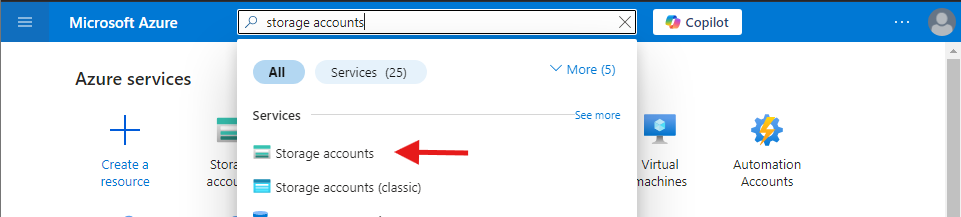
\includegraphics[width=0.8\textwidth]{img/1imm.png}
    \caption{Storage account zoekopdracht binnen de Azure Portal}
\end{figure}
Bij het aanmaken van het storage account kiezen we de correcte resource group, naam die het account moet krijgen, regio en bij redundancy kiezen we voor \texttt{Locally-redundant storage (LRS)}. Bij de optie \texttt{Account kind} kiezen we voor \texttt{General-purpose v2}, omdat deze versie alle benodigde functionaliteit biedt, zoals het ondersteunen van de blob storage en het configureren van immutability policies. 
\begin{figure}[h]
    \centering
    \captionsetup{justification=centering}    
    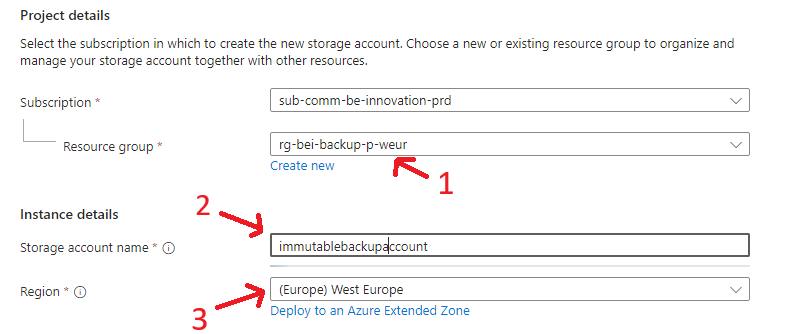
\includegraphics[width=0.8\textwidth]{img/3.1imm.png}
    \caption{Configuratie voor het nieuwe storage account}
\end{figure}
\begin{figure}[h]
    \centering
    \captionsetup{justification=centering}    
    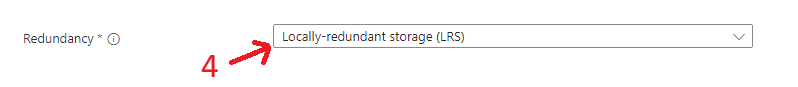
\includegraphics[width=0.8\textwidth]{img/3.2imm.png}
    \caption{Tweede deel van de configuratie voor het nieuwe storage account}
\end{figure}
\newpage
\subsubsection{Aanmaken van een container binnen het storage account}
Na het aanmaken van het storage account moet er een container geconfigureerd worden binnen het nieuwe storage account om de gegevens op te slaan. Bij het aanmaken van de container moet de \texttt{public access level} op private staan voor de veiligheid. Containers in Azure werken als mappen waarin je blobs kunt opslaan zoals back-ups.
\begin{figure}[h]
    \centering
    \captionsetup{justification=centering}    
    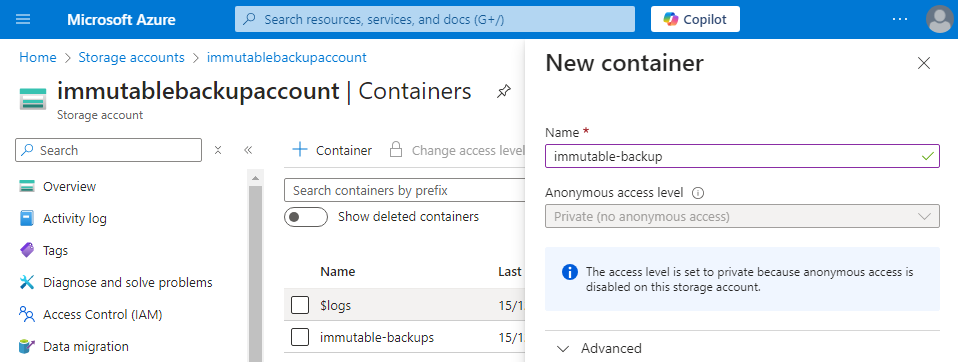
\includegraphics[width=0.8\textwidth]{img/4imm.png}
    \caption{Configuratie voor de container in het storage account}
\end{figure}
\subsubsection{Opzetten van een time-based retention policy}
Nadien moet er een immutability policy opgezet worden. Hierbij werd gekozen voor een time-based retention policy van 90 dagen, de back-up is met andere woorden bescherm tegen verwijdering of wijziging voor deze periode. Dit is een veilige en praktische keuze voor back-ups. Daarnaast is er bij de optie \texttt{ Allow protected append writes to } gekozen voor \texttt{ Block and append blobs}, dit maakt het mogelijk om gegevens te blijven toevoegen aan de blob zonder de bestaande gegevens te wijzigen of te verwijderen, wat ideaal is voor scenario's zoals logbestanden of incrementele back-ups.
\begin{figure}[h]
    \centering
    \captionsetup{justification=centering}    
    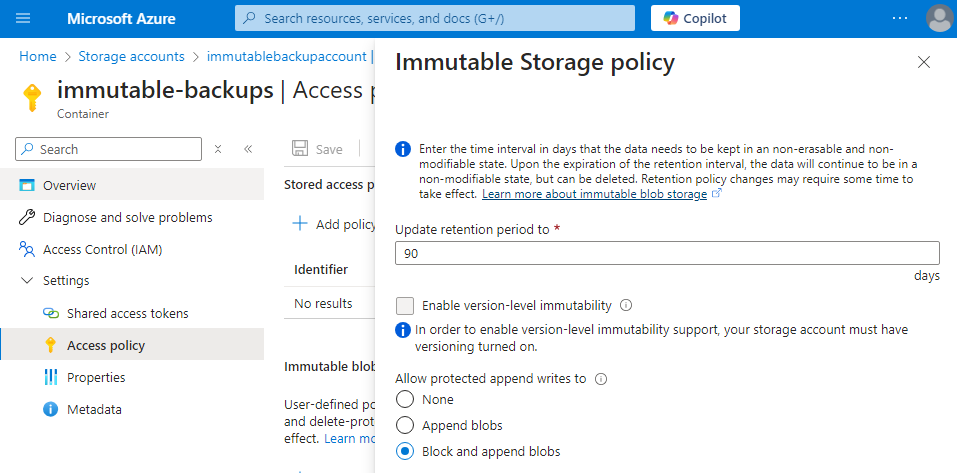
\includegraphics[width=0.8\textwidth]{img/6imm.png}
    \caption{Configuratie voor time-based retention policy}
\end{figure}
\newpage
\subsubsection{Testen van de immmutable storage}
Om de immutable storage te testen is er gekozen om een back-up van een MySQL-database de uploaden naar de container. Na het uploaden van het bestand was er geen optie om dit bestand te verwijderen of te wijzigen. Met andere woorden is deze back-up dus beschermd tegen een ransomware-aanval.
\begin{figure}[h]
    \centering
    \captionsetup{justification=centering}    
    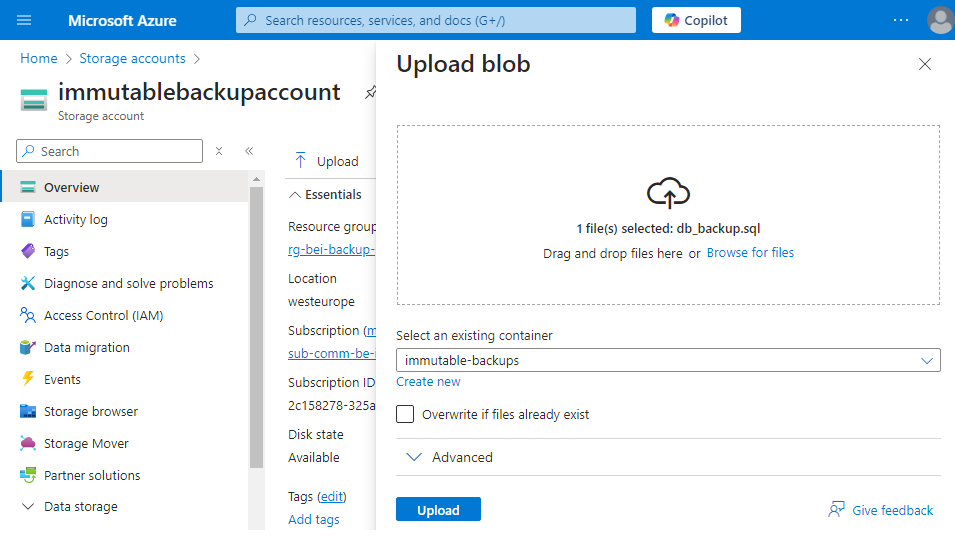
\includegraphics[width=0.8\textwidth]{img/7imm.png}
    \caption{Uploaden van het back-up bestand van de MySQL-databank}
\end{figure}
\begin{figure}[h]
    \centering
    \captionsetup{justification=centering}    
    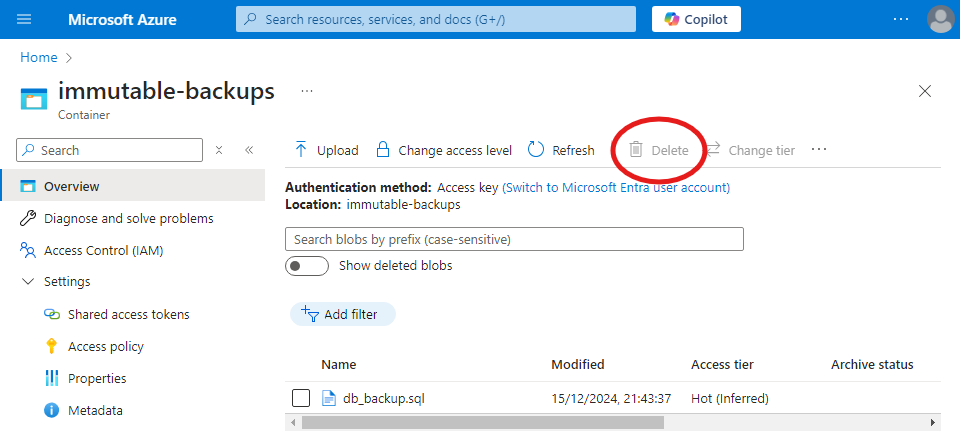
\includegraphics[width=0.8\textwidth]{img/8imm.png}
    \caption{Screenshot van de poging om het bestand te verwijderen, waarbij de actie wordt geblokkeerd}
\end{figure}
\subsubsection{Conclusie}
De implementatie van immutable storage op het azure storage account is succesvol afgerond, waardoor de opgeslagen back-ups nu beschermd zijn tegen onverwachte wijzigingen of verwijderingen. Daarnaast worden er dagelijks automatische back-ups van de databanken genomen, welke een retentieperiode van 7 dagen hebben. Dit zorgt ervoor dat er altijd een versie van de back-up beschikbaar is, zelfs als de meest recente back-up beschadigd of onbruikbaar blijkt. Deze combinatie van immutable storage en versiebeheer versterkt de bescherming tegen dataverlies en maakt het mogelijk om eerdere, werkende back-ups snel te herstellen.


\subsection{Implementatie van de Kubernetes-gebaseerde automatische back-upoplossing}

\subsubsection{Inleiding}
In dit deel wordt een Kubernetes-omgeving ingezet om een schaalbare en geautomatiseerde back-upoplossing te ontwikkelen voor PostgreSQL- en MySQL-databases. Voor testdoeleinden worden de databases lokaal gehost op een Vagrant Virtual Machine (VM), wat een geïsoleerde omgeving biedt voor het opzetten van de back-upworkflow. De productieomgeving van Forvis Mazars maakt echter gebruik van Azure, waardoor de lokale testomgeving het proces simuleert onder vergelijkbare principes.

De back-ups worden uitgevoerd door containers die draaien binnen Kubernetes Pods. Voor deze containers wordt gebruik gemaakt van een op maat gemaakte Docker-image. Deze image bevat een Python-script voor zowel het uitvoeren van de back-ups als het opschonen van verouderde bestanden. Kubernetes automatiseert de back-upworkflow verder met behulp van CronJobs, terwijl opslag wordt beheerd via Persistent Volumes (PV) en Persistent Volume Claims (PVC). Gevoelige gegevens worden beveiligd met Kubernetes Secrets.

\subsection{Relevantie van de Kubernetes-setup voor Forvis Mazars}

De Kubernetes-setup die in deze Proof of Concept (PoC) is ontwikkeld, blijkt direct relevant voor de werkomgeving van Forvis Mazars, aangezien ook daar Kubernetes wordt ingezet voor het beheer van de IT-infrastructuur. In deze sectie worden de overeenkomsten besproken, wordt toegelicht hoe de oplossing aansluit bij de behoeften van Forvis Mazars, en worden mogelijke aanpassingen beschreven om de setup volledig te integreren in hun bestaande workflows. Het belangrijkste verschil is dat bij Forvis Mazars de back-ups niet worden opgeslagen in een Persistent Volume, maar rechtstreeks worden geüpload naar een Azure Storage Container.

\subsubsection*{Overeenkomsten met de Forvis Mazars Setup}

Bij Forvis Mazars wordt gebruikgemaakt van Kubernetes Pods om databases te beheren en back-ups te genereren. De belangrijkste onderdelen van de ontwikkelde oplossing, zoals het gebruik van CronJobs en containerisatie, komen sterk overeen met de gebruikte werkwijze. Dit zorgt ervoor dat Forvis Mazars deze oplossing met minimale aanpassingen kan overnemen. Dit zijn de voornaamste gelijkenissen tussen de uitgewerkte oplossing en de productieomgeving van Forvis Mazars:

\begin{itemize}
    \item \textbf{Automatisering via CronJobs} \\
    Bij zowel de PoC als de setup van Forvis Mazars worden Kubernetes CronJobs toegepast voor het plannen van taken. In de PoC worden deze CronJobs ingezet om dagelijkse back-ups uit te voeren en oudere back-ups automatisch te verwijderen. Deze aanpak wordt gekenmerkt door schaalbaarheid en sluit goed aan bij de architectuur van Kubernetes die door Forvis Mazars wordt gebruikt.
    
    \item \textbf{Beveiliging van wachtwoorden} \\
    In de PoC worden Kubernetes Secrets gebruikt om gevoelige informatie, zoals databasewachtwoorden, door te geven aan het Python-script dat de back-ups uitvoert. Dit zorgt ervoor dat wachtwoorden niet hardcoded hoeven te worden in configuratiebestanden of scripts. Hoewel niet bekend is of Forvis Mazars eveneens Secrets gebruikt, biedt deze aanpak een veilige en flexibele oplossing die eenvoudig kan worden geïntegreerd in een vergelijkbare omgeving.
    
    \item \textbf{Schaalbaarheid en containerisatie} \\
    Het gebruik van een gestandaardiseerde Docker-image voor de uitvoering van de back-ups weerspiegelt de wijze waarop Kubernetes Pods bij Forvis Mazars worden beheerd. Containers kunnen eenvoudig worden aangepast of opnieuw worden ingezet, zonder dat dit aanpassingen aan de volledige infrastructuur vereist.
\end{itemize}


\subsubsection*{Verschil in Back-upopslag}

Het grootste verschil tussen de PoC en de setup van Forvis Mazars ligt in de wijze van back-upopslag. Bij de PoC worden back-ups lokaal opgeslagen in een Persistent Volume (PV), terwijl deze bij Forvis Mazars direct worden geüpload naar een Azure Storage Container. Dit verschil heeft enkele belangrijke implicaties:

\begin{itemize}
    \item \textbf{Opslaglocatie} \\
    Persistent Volumes bieden een eenvoudige manier om gegevens lokaal binnen een Kubernetes-cluster op te slaan. Dit maakt ze geschikt voor testomgevingen en lokale implementaties, zoals in de PoC. Forvis Mazars maakt echter gebruik van een cloudopslagoplossing in de vorm van Azure Storage Containers. Deze oplossing biedt voordelen zoals schaalbaarheid, hoge beschikbaarheid en eenvoud in beheer binnen een productieomgeving.
    
    \item \textbf{Integratie met Azure} \\
    Bij Forvis Mazars wordt de Kubernetes-setup geïntegreerd met Azure door gebruik te maken van tools zoals Azure CLI of SDK’s voor het uploaden van back-ups naar Azure Storage. Binnen de PoC zou een vergelijkbare integratie kunnen worden gerealiseerd door het Python-script aan te passen, zodat back-ups direct naar Azure worden geüpload in plaats van lokaal te worden opgeslagen. Dit kan worden bereikt door de Azure Storage SDK voor Python te implementeren of CLI-opdrachten toe te voegen aan de Docker-image.
\end{itemize}

Door deze overeenkomsten en verschillen te analyseren, kan worden geconcludeerd dat de ontwikkelde Kubernetes-setup een solide basis biedt die volledig kan worden afgestemd op de operationele vereisten van Forvis Mazars.

\subsubsection{Python-script voor databaseback-ups}
Het Python-script, zie bijlage \ref{sec:python}, is ontworpen om automatisch back-ups te maken van MySQL- en PostgreSQL-databases en biedt tevens functionaliteit om oude back-ups te verwijderen op basis van een ingestelde retentieperiode. Daarbij zorgt het script voor versiebeheer van de back-ups door in de bestandsnaam de datum en het type database op te nemen, wat het mogelijk maakt om verschillende versies van de back-ups te onderscheiden op basis van de tijd waarop ze zijn gemaakt.  Het maakt gebruik van een object-georiënteerde aanpak, waarbij de \texttt{Backup}-klasse de kern van het script vormt. Bij de initialisatie van de klasse worden verschillende parameters ingesteld, waaronder de naam van de database, de gebruikersnaam en het type database (MySQL of PostgreSQL), evenals de locatie van de back-ups. De bestandsnaam voor de back-up wordt dynamisch gegenereerd op basis van de datum en het type database, en krijgt de vorm van \texttt{backup-\{type\}-\{YYYY-MM-DD\}-\{database\_name\}.dump}. Daarnaast worden omgevingsvariabelen gebruikt voor de IP-adressen van de servers waarop de databanken draaien en poorten van zowel MySQL als PostgreSQL, wat zorgt voor een flexibele configuratie van het script.

\begin{lstlisting}[language=script, caption={Backup-klasse van het python-script.}]
class Backup:
def __init__(self, database_name, database_user, type, backup_dir):
timestr = datetime.datetime.now().strftime('%Y-%m-%d')
self.filename = f'backup-{type}-{timestr}-{database_name}.dump'
self.database_name = database_name
self.database_user = database_user
self.type = type
self.password = None
self.backup_dir = backup_dir
self.hostname_mysql = os.environ.get("HOSTNAME_MYSQL", "192.168.1.62")
self.hostname_psql = os.environ.get("HOSTNAME_PSQL", "192.168.1.62")
self.port_mysql = os.environ.get("PORT_MYSQL", "3306")
self.port_psql = os.environ.get("PORT_PSQL", "5432")
\end{lstlisting}

Een essentieel onderdeel van het script is de \texttt{set\_password}-methode, die het databasewachtwoord uit een omgevingsvariabele haalt. Indien het wachtwoord niet is ingesteld, wordt een waarschuwingsbericht weergegeven en stopt het script om onveilige of onvolledige back-ups te voorkomen. Dit maakt de back-upprocedure veiliger en garandeert dat alleen bevoegde gebruikers toegang hebben tot de databasegegevens.

De \texttt{create\_backup}-methode is verantwoordelijk voor het daadwerkelijk uitvoeren van de back-up. Afhankelijk van het type database wordt ofwel het \texttt{mysqldump}-commando voor MySQL of het \texttt{pg\_dump}-commando voor PostgreSQL uitgevoerd. Bij het maken van een MySQL-back-up wordt het \texttt{mysqldump}-commando gebruikt met de juiste databasegegevens, zoals gebruikersnaam, wachtwoord, hostnaam en poort. Voor PostgreSQL wordt het \texttt{pg\_dump}-commando gebruikt, waarbij de uitvoer in het "custom format" wordt opgeslagen. Beide commando’s worden uitgevoerd via de \texttt{subprocess.run}-functie, die de uitvoer naar een bestand schrijft. Mocht een van de commando's mislukken, dan zorgt de foutafhandeling ervoor dat het script stopt en een foutmelding wordt weergegeven.
\begin{lstlisting}[language=script, caption={create\_backup-methode van het python-script.}]
    def create_backup(self, type):
    # Create a backup of the database.
    
    # Ensure the backup directory exists
    if not os.path.exists(self.backup_dir):
    os.makedirs(self.backup_dir)
    # Prepend the backup directory to the filename
    full_path = os.path.join(self.backup_dir, self.filename)
    
    if type == "MYSQL":
    try:
    cmd = [
    'mysqldump',
    '--single-transaction',
    '-u', self.database_user,
    f'-p{self.password}',
    '-h', self.hostname_mysql,
    '-P', str(self.port_mysql),
    '--no-tablespaces',
    '-B', self.database_name,
    ]
    with open(full_path, 'w') as backup_file:
    result = subprocess.run(cmd, stdout=backup_file, check=True)  # nosec
    if result.returncode != 0:
    logging.warning(f'Command failed. Return code: {result.returncode}')
    exit(1)
    return full_path
    except Exception as e:
    logging.warning(e)
    exit(1)

    elif type == "PSQL":
    try:
    cmd = [
    'pg_dump',
    '-U', self.database_user,
    '-h', self.hostname_psql,
    '-p', str(self.port_psql),
    '-F', 'c',
    '-f', full_path,
    self.database_name
    ]
    result = subprocess.run(cmd, check=True)  # nosec
    if result.returncode != 0:
    logging.warning(f'Command failed. Return code: {result.returncode}')
    exit(1)
    return full_path
    except Exception as e:
    logging.warning(e)
    exit(1)
\end{lstlisting}

Daarnaast bevat het script de \texttt{delete\_old\_backups}-methode, die ervoor zorgt dat oude back-ups automatisch worden verwijderd om opslagruimte te beheren. Het script vergelijkt de wijzigingsdatum van elk bestand in de opgegeven back-up directory met de huidige datum en verwijdert bestanden die ouder zijn dan de ingestelde retentieperiode. Dit maakt het mogelijk om ongewenste en verouderde back-ups op te schonen, wat belangrijk is voor het beheer van systeembronnen.
\begin{lstlisting}[language=script, caption={delete\_old\_backups-methode van het python-script.}]
    @staticmethod
    def delete_old_backups(directory, retention_days):
    """
    Deletes backup files older than the specified retention period.
    """
    now = datetime.datetime.now()
    logging.info(f"Starting cleanup of backups in {directory} with retention period: {retention_days} days")
    for file in os.listdir(directory):
    if file.startswith("backup-") and file.endswith(".dump"):
    file_path = os.path.join(directory, file)
    file_mtime = datetime.datetime.fromtimestamp(os.path.getmtime(file_path))
    age = (now - file_mtime).days
    logging.info(f"Checking file {file_path}: age = {age} days")
    if age >= retention_days:
    try:
    os.remove(file_path)
    logging.info(f"Deleted old backup: {file_path}")
    except Exception as e:
    logging.warning(f"Failed to delete {file_path}: {e}")
    else:
    logging.info(f"File {file_path} is not old enough to delete (age = {age} days).")
\end{lstlisting}

Het script maakt gebruik van uitgebreide logging om de voortgang van de back-up- en opruimprocessen te documenteren. Logging biedt inzicht in de status van de uitgevoerde handelingen, zoals succesvolle back-ups, waarschuwingen voor ontbrekende omgevingsvariabelen, foutmeldingen bij mislukte bewerkingen en informatie over de bestanden die worden gecontroleerd of verwijderd.

Ten slotte wordt het script uitgevoerd vanuit de \texttt{main}-functie, die de ingevoerde argumenten verwerkt en de bijbehorende methoden aanroept. Als een back-up wordt aangevraagd, wordt een instantie van de \texttt{Backup}-klasse gemaakt en worden de methoden \texttt{set\_password} en \texttt{create\_backup} uitgevoerd. Als de gebruiker de optie voor het verwijderen van oude back-ups heeft opgegeven, wordt de statische methode \texttt{delete\_old\_backups} aangeroepen om de oude bestanden te verwijderen. Op deze manier biedt het script een oplossing voor het beheren van back-ups en het efficiënt verwijderen van verouderde back-ups.

\subsubsection{Dockerfile}
Het Dockerfile, zoals weergegeven in bijlage \ref{sec:dockerfile}, is ontworpen om een container te creëren die de benodigde software bevat voor het uitvoeren van de geautomatiseerde back-ups via het eerder besproken Python-script binnen Kubernetes. Het begint met het ophalen van de laatste versie van Ubuntu als basisimage. Vervolgens worden de MySQL- en PostgreSQL-clients geïnstalleerd, samen met Python3 voor het uitvoeren van het script. Het Python-script wordt vanuit de lokale src-map naar de container gekopieerd. Deze Docker-image is uiteindelijk gepushed naar een Docker-account, zodat deze gebruikt kan worden in de Kubernetes-omgeving. Dit Dockerfile biedt de nodige omgeving voor het uitvoeren van de back-ups in de Kubernetes pods.


\subsubsection{Kubernetes cronjobs en werking}
Een Kubernetes Pod is de kleinste uitvoereenheid binnen een Kubernetes-cluster. Elke Pod bevat een of meer containers die een specifieke taak uitvoeren. In dit project wordt een Pod geconfigureerd om:
\begin{itemize}
    \item De back-up van een database uit te voeren.
    \item Data op te slaan in een Persistent Volume.
    \item Gevoelige informatie, zoals wachtwoorden, te beheren via Secrets.
\end{itemize}

Voor elke database (PostgreSQL en MySQL) is een aparte CronJob geconfigureerd. Deze CronJobs maken gebruik van dezelfde Docker-image, maar passen specifieke parameters toe om de juiste database te back-uppen.

Het proces verloopt als volgt:
\begin{enumerate}
    \item De CronJob wordt volgens een gepland tijdschema uitgevoerd.
    \item De CronJob spint een Pod op waarin de container draait die de back-up uitvoert.
    \item De container voert het Python-script uit dat de database-back-up naar een Persistent Volume schrijft.
    \item Na voltooiing wordt de Pod beëindigd, terwijl de back-upbestanden bewaard blijven.
\end{enumerate}

Het eerste CronJob YAML-bestand, dat wordt gepresenteerd in bijlage \ref{sec:cron}.1,  configureert een geautomatiseerde taak die elke nacht om 2 uur een back-up maakt van een MySQL-database. Deze taak wordt uitgevoerd in een Kubernetes-omgeving en maakt gebruik van een container die het eerder genoemde Python-script uitvoert om de back-up te maken. De cronjob is opgezet om periodiek de database te back-uppen zonder menselijke tussenkomst.

De \texttt{apiVersion: batch/v1} en \texttt{kind: CronJob} geven aan dat het bestand een Kubernetes CronJob definieert, een soort geplande taak die op regelmatige tijdstippen wordt uitgevoerd. De \texttt{schedule} is ingesteld op "0 2 * * *", wat betekent dat de back-up elke dag om 2:00 uur 's nachts wordt uitgevoerd. Dit schema volgt de standaard cron-vergelijkingsnotatie, waarbij de tijd en frequentie worden gedefinieerd.

Binnen de \texttt{jobTemplate} wordt de daadwerkelijke taak gespecificeerd die door de cronjob moet worden uitgevoerd. De container die wordt gebruikt voor deze taak is de \texttt{bouzewazi/ubu4} Docker-image, die het Python-script bevat dat verantwoordelijk is voor het maken van de back-up. Het script wordt uitgevoerd met een aantal argumenten, waaronder de database-naam (\texttt{testdb}), gebruikersnaam (\texttt{root}), het type database (\texttt{MYSQL}), en de locatie van de back-up (\texttt{/data}). Dit zorgt ervoor dat de juiste database op het juiste moment wordt geback-upt en de back-up wordt opgeslagen in een gedeelde opslaglocatie.

De container maakt gebruik van een persistent volume claim, gedefinieerd onder \texttt{volumes}, om back-upbestanden op te slaan. Het volume wordt gekoppeld aan een specifieke directory binnen de container via \texttt{volumeMounts}. Dit zorgt ervoor dat de opgeslagen gegevens behouden blijven, zelfs als de container opnieuw wordt opgestart.

Verder wordt het databasewachtwoord veilig doorgegeven via een Kubernetes Secret. Het wachtwoord wordt opgehaald uit een Kubernetes Secret als een environment variable genaamd \texttt{DB\_PASSWORD}. Dit zorgt ervoor dat gevoelige gegevens op een veilige manier aan de container worden verstrekt zonder dat ze hard-coded in de YAML worden opgenomen.

Daarbij is er ook een andere CronJob die dezelfde functionaliteit biedt, maar dan voor het maken van back-ups van een PostgreSQL-database. Deze CronJob is vergelijkbaar met de MySQL CronJob, met aanpassingen die specifiek zijn voor de PostgreSQL-databaseconfiguratie, zoals te zien in bijlage \ref{sec:cron}.2.

Tenslotte is er een CronJob die oude back-ups verwijdert die ouder zijn dan 14 dagen, wat de retentieperiode is voor de dagelijkse back-ups. Dit zorgt ervoor dat alleen back-ups binnen de laatste 14 dagen bewaard blijven, waardoor opslag efficiënt wordt beheerd, zoals beschreven in bijlage \ref{sec:cron}.3.

\subsubsection{Overstap van Docker naar Kubernetes voor cronjob automatisering}
Aanvankelijk werd gekozen om de automatisering van de back-ups te beheren via een Docker-container, waarin CronJobs werden ingesteld om dagelijks back-ups te maken en oude back-ups te verwijderen. Binnen de container werd een setup.sh-script uitgevoerd om de cron-service te starten en de benodigde cronjobs te configureren. Dit proces gebruikte een Dockerfile, zie bijlage \ref{sec:dockerfile}.2, die de benodigde software installeerde, zoals MySQL-client, PostgreSQL-client, cron en Python3. Ook werd het Python-script en setup-script, zie bijlage \ref{sec:setup}, in de container gekopieerd. De CronJobs werden geconfigureerd om dagelijks back-ups te maken om 2:00 uur 's nachts en oude back-ups, ouder dan 14 dagen, te verwijderen.

Hoewel dit functioneel was, bood deze oplossing beperkte persistentie voor de back-ups, aangezien de opslag binnen de container plaatsvond. Uiteindelijk werd besloten om de CronJobs op Kubernetes te draaien, wat beter aansluit bij de infrastructuur van Forvis Mazars. Kubernetes biedt schaalbaarheid, persistente opslag en een efficiënte integratie binnen de bestaande setup van het bedrijf, waardoor het de logische keuze was voor het beheren van de geautomatiseerde back-uptaken.

\subsection{Herstelcapaciteit (Restore from Backup)}
Een belangrijk onderdeel van het praktijkgedeelte van dit onderzoek is het testen van de herstelcapaciteit (restore from back-up). Dit was een essentiële vereiste in het onderzoek, waarbij de focus lag op het efficiënt en snel herstellen van systemen vanuit de back-ups. Het doel was om een idee te krijgen over hoe snel en betrouwbaar een databank up-and-running kan zijn na het ondergaan van een incident.

Voor deze must-have werd het herstelproces gesimuleerd in een testomgeving waarbij de back-ups werden opgehaald uit de immutable Azure storage container en deze dan herstelt werden in een MySQL- en PostgreSQL-databank. Deze testomgeving komt grotendeels overeen met de actieve omgeving die Forvis Mazars gebruikt. Het proces omvatte de volgende stappen:

\subsubsection{Back-ups ophalen uit de immutable storage in Azure}
De back-ups werden veilig opgeslagen in een Azure Storage Account met een immutable opslagbeleid, wat een cruciale maatregel is tegen ransomware-aanvallen. Door het gebruik van het \texttt{az storage blob download}-commando werden de back-ups gedownload naar de lokale virtuele machine.

\subsubsection{Herstellen van de PostgreSQL- en MySQL-databanken}
Na het downloaden werden de PostgreSQL- en MySQL-databases opnieuw opgezet met herstelcommando’s. Voor PostgreSQL werd het bestand hersteld met \texttt{pg\_restore}, terwijl voor MySQL gebruik werd gemaakt van het \texttt{mysql}-commando. Beide hersteltaken verliepen succesvol en zonder dataverlies. Om aan te tonen dat de integriteit van de back-up is behouden werd er een hash berekend van de tabel in de MySQL-shell van de database voor de restore en deze werd vergeleken met de hash na het herstellen van de database vanuit de back-up. Dit is de hash van de database voor de restore:
\begin{lstlisting}[language=code, caption={MySQL commando om de hash van de tabel te berekenen voor de restore.}]
mysql> SELECT SUM(CRC32(CONCAT_WS('#', firstName, lastName, gender, address, phone, email))) AS checksum FROM testdb;
+---------------+
| checksum      |
+---------------+
| 4336568446292 |
+---------------+
1 row in set (0.00 sec)
\end{lstlisting}  
De hash van de database na het uitvoeren van de restore is identiek en geeft dezelfde output:
\begin{lstlisting}[language=code, caption={MySQL commando om de hash van de tabel te berekenen voor de restore.}]
mysql> SELECT SUM(CRC32(CONCAT_WS('#', firstName, lastName, gender, address, phone, email))) AS checksum FROM testdb;
+---------------+
| checksum      |
+---------------+
| 4336568446292 |
+---------------+
1 row in set (0.00 sec)
\end{lstlisting}  

Dit hele proces is gemeten en duurde 48 seconden, wat wijst op een snelle toegang tot de back-ups in noodsituaties. Het back-upbestand voor de MySQL-databank had een bestandsgrootte 383 KiB en het bestand voor de PostgreSQL-databank had een grootte van 45,16 KiB. Deze bestanden werden gedownload met een internetsnelheid van 75.33 Mbit/s. Dit is getest met de tool speedtest-cli.


\subsubsection{Link met Herstelcapaciteit}
De testprocedure toont aan dat de opgestelde back-upstrategie niet alleen effectief is in het beschermen van gegevens, maar ook voldoet aan de eisen van herstelcapaciteit:

\begin{itemize}
    \item \textbf{Efficiëntie:} Het herstelproces, vanaf het downloaden van de back-ups tot het opnieuw opzetten van de databases, verliep in een relatief korte tijd. Dit bevestigt dat de back-ups eenvoudig en snel toegankelijk zijn, wat essentieel is in een bedrijfsomgeving waar down-time zo laag mogelijk moet zijn.
    
    \item \textbf{Betrouwbaarheid:} Door gebruik te maken van immutable opslag in Azure worden de back-ups beschermd tegen ongewenste acties en aanvallen, wat de kans op succesvol herstel sterk verhoogt.
\end{itemize}

\subsubsection{Conclusie}
De uitgevoerde tests bieden waardevolle inzichten in de herstelcapaciteit van de back-upstrategie. Het toont aan hoe een goed ontworpen back-upplan bedrijven in staat stelt om snel te reageren op noodsituaties en hun systemen betrouwbaar te herstellen. Hiermee is aangetoond dat het systeem niet alleen beschermt tegen gegevensverlies, maar ook operationeel herstel mogelijk maakt binnen een acceptabele tijd. Dit maakt het een reële oplossing voor bedrijven die ransomware-resistente back-upstrategieën willen implementeren.































